\chapter{Background Theory}

\label{ch:background}

Plasma is often described as the fourth state of matter. It has similar characteristics to gases, where it is compressible and does not conform to a specific shape; however the key difference is that plasmas are highly electrically conductive, even capable of producing it’s own magnetic field. This is because plasmas contain a large number of positive ions that interact in a ``sea" of disassociated free-moving electrons.

\section{Plasma Discharge}

Plasma are generated in one of two primary ways. The first is via extreme heating of a gas whereby the electrons gain sufficient energy to escape the electromagnetic force of the nucleus. The most obvious example of this is in stars where interstellar gas clouds collapse and form a plasma for nuclear fusion. The other method, which is the main focus of this report, is the exposure of a gas to a large voltage difference. This in turn ignites the plasma in a process described in the rest of this chapter. An everyday example of this is lightning, where  charges build up between the clouds to the ground, which in turn causes the potential difference between the two to grow until the air in between breaks down.

\subsection{Paschen's Law}

The voltage necessary to breakdown a gas is given by Paschen's law. It states that breakdown voltage is a function of two parameters \cite{Lieberman2005}: the pressure of the gas and the distance between the electrodes, referred to as the gap length. Specifically, the breakdown voltage is given by the product of these two parameters.

In order for a breakdown to occur, there needs to be a small number of electrons already present in the gas. This can be caused internally by a smaller number of already excited gas molecules, or externally by light entering the gas chamber disassociating electrons. Then by applying a voltage, these electrons gain energy creating other electrons from ionising collisions. When more electrons are generated from the collisions than are lost, an avalanche is created, which causes the gas breakdown.

The voltage breakdown can expressed by the following equation \cite{Lieberman2005}:

\begin{equation}
	V_B = \frac{B \rho d}{ln(A \rho d) - ln[ln(1-\frac{1}{\gamma_{se}})]}
\end{equation}

where $V_B$ is the breakdown voltage, $\rho$ is the pressure of the gas, $d$ is the gap length, $\gamma_{se}$ is a coefficient for secondary-electron emissions (explained in section 2.1.2), and $A$ and $B$ are constants for a given that are determined experimentally.

However it much easier to understand Paschen's law pictorially. Figure \ref{fig:pashen_curve} illustrates the voltage breakdown curves across various gases. Each curve is slightly different, however all of them do exhibit the shape of a parabola. Supposing if:

\begin{itemize}
	\item\textbf{The gap length remains constant}. Starting with a large pressure, the mean free path of an electron within the gas is low, meaning it does not have sufficient time to gain enough energy to cause an ionising collisions with neutral gas. As the pressure is then reduced, the mean free path increases, making it easier for the electrons to generate ionising collisions; until a certain critical pressure that is. Beyond this, decreasing the pressure further decreases the likelihood of an electron colliding with a neutral gas particle.

	\item\textbf{The pressure remains constant}. When the gap length is very small, the electrons do no have sufficient time to accelerate the energy required to ionise the background gas. Increasing the gap to a certain point gives the electrons sufficient time to gain the energy required for ionisation. However, as the gap length continues to be increased, the electric field between the electrodes decreases, hence the electrons do not have enough energy to cause ionising collisions.
\end{itemize}

\begin{figure}[h!]
	\centering
	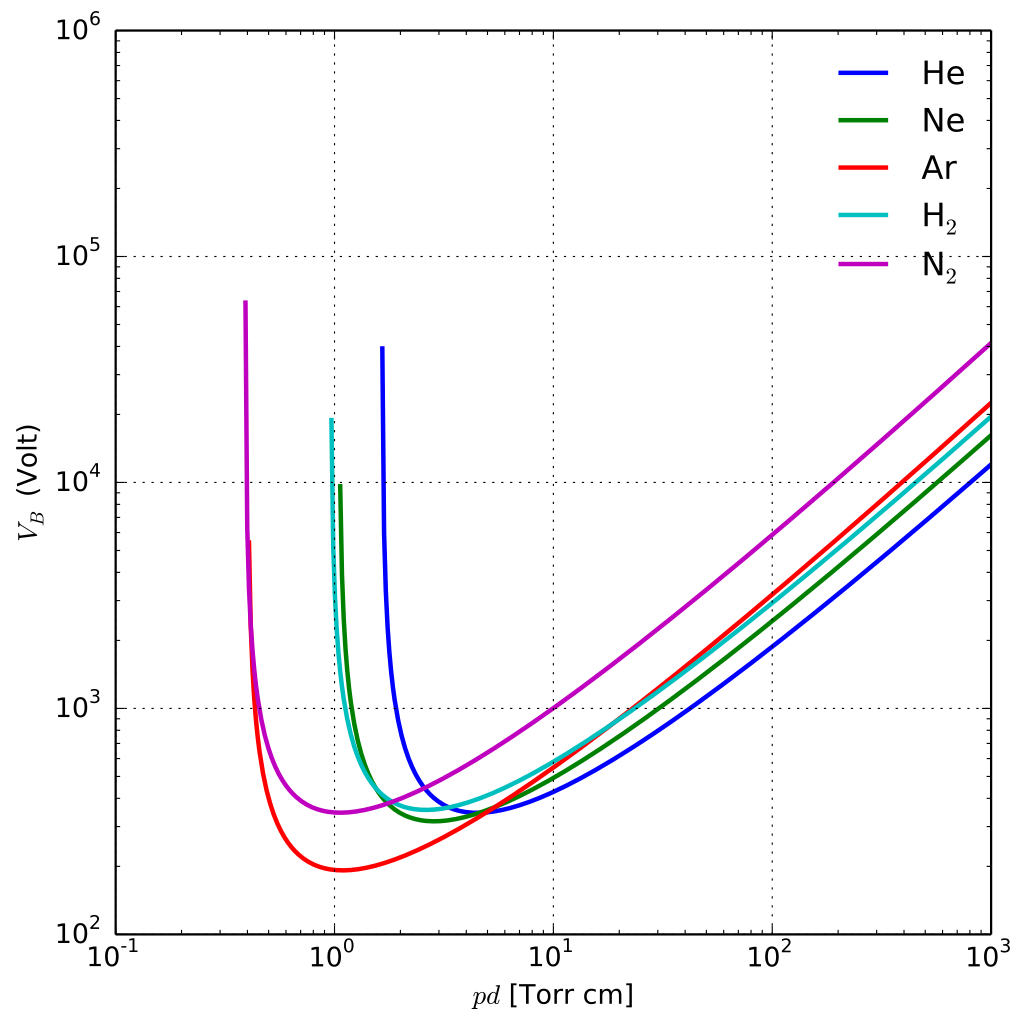
\includegraphics[width=0.6\linewidth]{background/figures/paschen_curve.png}
	\caption{Paschen curve for Helium, Neon, Argon, Hydrogen, and Nitrogen gases \cite{Lieberman2005}.}
	\label{fig:pashen_curve}
\end{figure}

% One thing to note about Paschen’s law is that it is loses its accuracy for smaller gap lengths, below 10 to 15 um. The model incorrectly predicts that the voltage breakdown rises towards infinity; however in reality, there is an initial increase before it decreases again. 


\subsection{DC Discharge}

Consider a circuit as seen in figure \ref{fig:basic_circuit}. Two parallel electrodes with a DC voltage applied, and a neutral gas contained within a chamber. A the resistance of the variable resistor is decreased, which in turn increases the current through the plasma, one would observe three distinct discharge regions \cite{Gudmundsson2017}.

\begin{figure}[h!]
	\centering
	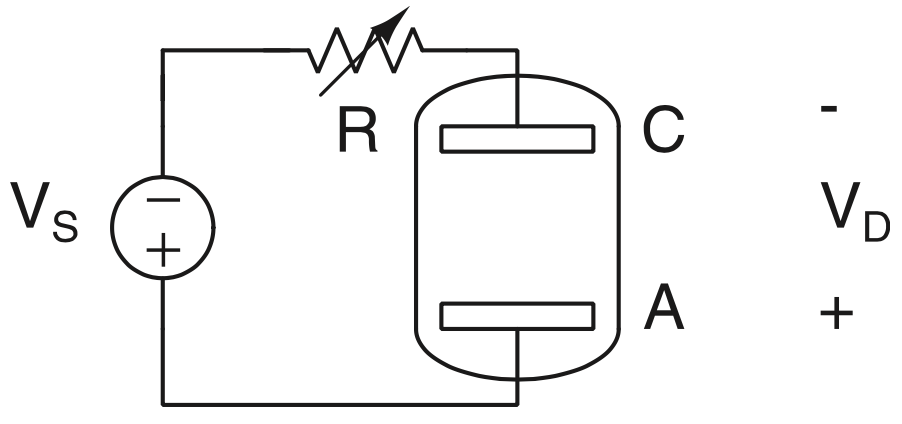
\includegraphics[width=0.6\linewidth]{background/figures/basic_circuit.png}
	\caption{Circuit diagram with a source voltage ($V_s$) and variable resistor ($R$) to control the current through a discharge region ($C$ to $A$) \cite{Gudmundsson2017}.}
	\label{fig:basic_circuit}
\end{figure}

The first, is the dark discharge (or sometime referred to as the Townsend discharge) region. Initially, the voltage between the electrodes builds up as the only current through the plasma is caused by pre-existing electrons, say from cosmic radiation; however this current quickly saturates. Then, once the electrons gain sufficient energy, they begin colliding with the background gas to produce additional electrons in a process called the \textit{Townsend avalanche}. Once this avalanche is self-sustaining, the voltage breakdown of the gas is achieved.

\begin{figure}[h!]
	\centering
	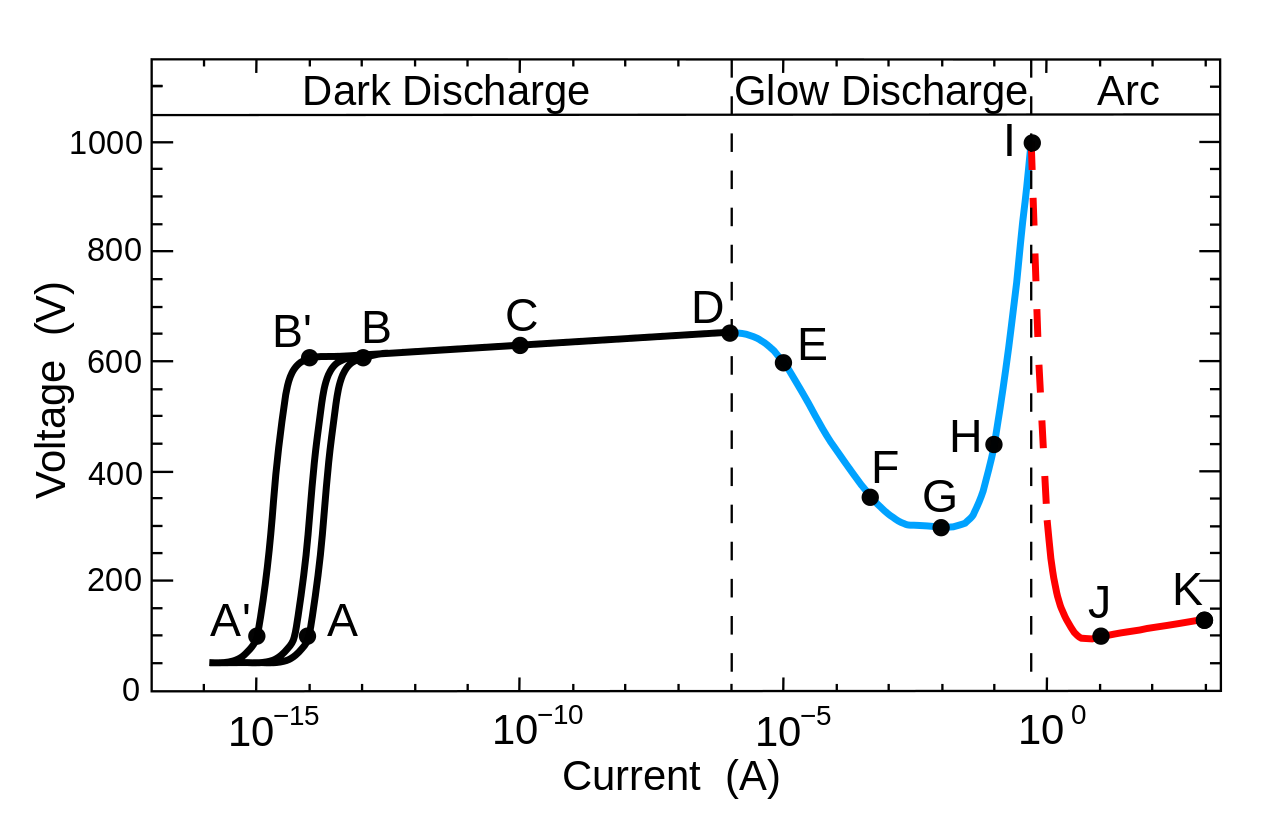
\includegraphics[width=0.8\linewidth]{background/figures/dc_discharge.png}
	\caption{Depiction of the current-voltage relationship across three discharge regions \cite{Gallo1975}.}
	\label{fig:dc_discharge}
\end{figure}

After the breakdown, the plasma is said to be in a glow discharge region. Here, the voltage across the plasma decreases since a transition from a gas to plasma state causes a decrease in resistance, implying that the ionisation process from the avalanche is more efficient. This efficiency stems from the fact that the electrons are generated by a secondary means in addition to the standard Townsend avalanche. This process is called the secondary emission of electrons, which is caused the energetic collisions of ions or metastable with the surface of the cathode. These \textit{secondary-electrons} are then accelerated by the electric field and cause further Townsend avalanches.

At first, ion bombardment on the surface of the cathode is non-uniform but as the current generated from this increases, it eventually stabilises and distribution of the plasma (and thus the ions) across the cathode become more uniform. This is referred to as \textit{subnormal glow} and \textit{normal glow} respectively. As the current is increased further, ion bombardment across the cathode becomes saturated as it covers the entire surface of the cathode. This is referred to as \textit{abnormal glow}, and increasing the current further causes the glow discharge to become an arc.

In the arc discharge region, the ion bombardments onto the cathode cause the cathode to heat up to a point where electrons are generated via thermionic radiation. This significantly reduces the resistance of the plasma, causing a very large drop of the voltage. 

For the purposes of this project, all plasma will be operating in the glow discharge region. The reason being, operating beyond the point abnormal glow increases the sputtering rate. \textit{Sputtering} is the ejections of ions from the cathode caused by the ion bombardment process. While useful for processes such as ion etching \cite{Lieberman2005}, sputtering would not be favourable for the application of a plasma cathode electron gun as the consumption of the cathode is something to be eliminated. Sputtering has the additional downside of potentially contaminating the final print as ejected atoms could end up in the electron beam. 

\begin{figure}[h!]
	\centering
	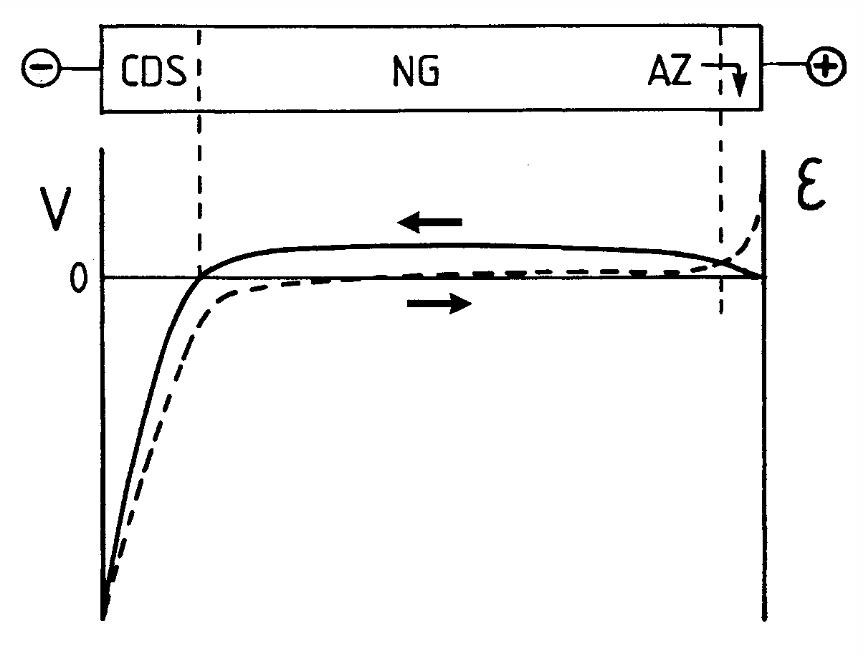
\includegraphics[width=0.7\linewidth]{background/figures/glow_discharge.png}
	\caption{Schematic highlighting the regions present in a DC glow discharge \cite{Bogaerts2002}. The cathode is on the left and the grounded anode is on the right. (CDS is the cathode dark space, NG is the negative glow, and AZ is the anode dark space.}
	\label{fig:glow_discharge}
\end{figure}

In a glow discharge there are typical three spatial regions present. These include a \textit{cathode dark space}, a \textit{negative glow} region, and the \textit{anode dark space} \cite{Gudmundsson2017, Bogaerts2002}. This can be observed in figure \ref{fig:glow_discharge}, that shows the potential difference in each region. Do note, as the distance between the electrodes is increased, additional regions may develop, however these three regions will always persist. The dark space regions are called \textit{sheaths} while the negative glow region is known as the \textit{bulk plasma}. Generally, the sheaths on the cathode will be much larger than that of the anode, as it corresponds to the region where electrons are being accelerated before gaining sufficient energy to cause ionising collisions. In contrast, the anode sheaths are caused by electrons colliding with the anode, thus creating a region of positive charge which repel any ions to the bulk plasma. Finally, the bulk plasma is the quasi-neutral region that contains the ions and electrons of the plasma.


\subsection{AC Discharge}

If the voltage source in the circuit of figure \ref{fig:basic_circuit} were to be replaced with a low frequency AC source, the discharge behaviour would be effectively identical to that of the DC discharge. This is provided that the half time period of an AC cycle is larger than the duration for ions and electrons to move across the electrodes \cite{Bogaerts2002}.

However, as the frequency of the AC source is increased, typically to the region of radio or microwave frequencies, there is an asymmetry between the movement of the ions and electrons. The electrons are capable of responding to the change in the electric fields relatively quickly; however, due to the ions being significantly heavier than electrons, they have a much slower response time hence are restricted to their inertia \cite{Chabert2011}.

Since the ions cannot respond to the changing electric field quick enough, the generation of electrons via the process of secondary-emissions is minimal. Instead what occurs is that electrons begin accelerating through the bulk plasma towards the anode during the first half period of the AC signal. Then as the direction of the electric field reverses in the second half period of the signal, the positions of the anode and cathode flip, and any electron that has not collided with the original anode (which is now the cathode), gets accelerated through the bulk plasma towards the new anode. This oscillating behaviour increases the likelihood of ionising collisions with the neutral background gas. As the frequency of the AC source is increased, more electrons become trapped in this regime, hence it is no surprise that the breakdown voltage of the plasma decreases \cite{Chu1992}.

 
\begin{figure}[h!]
	\centering
	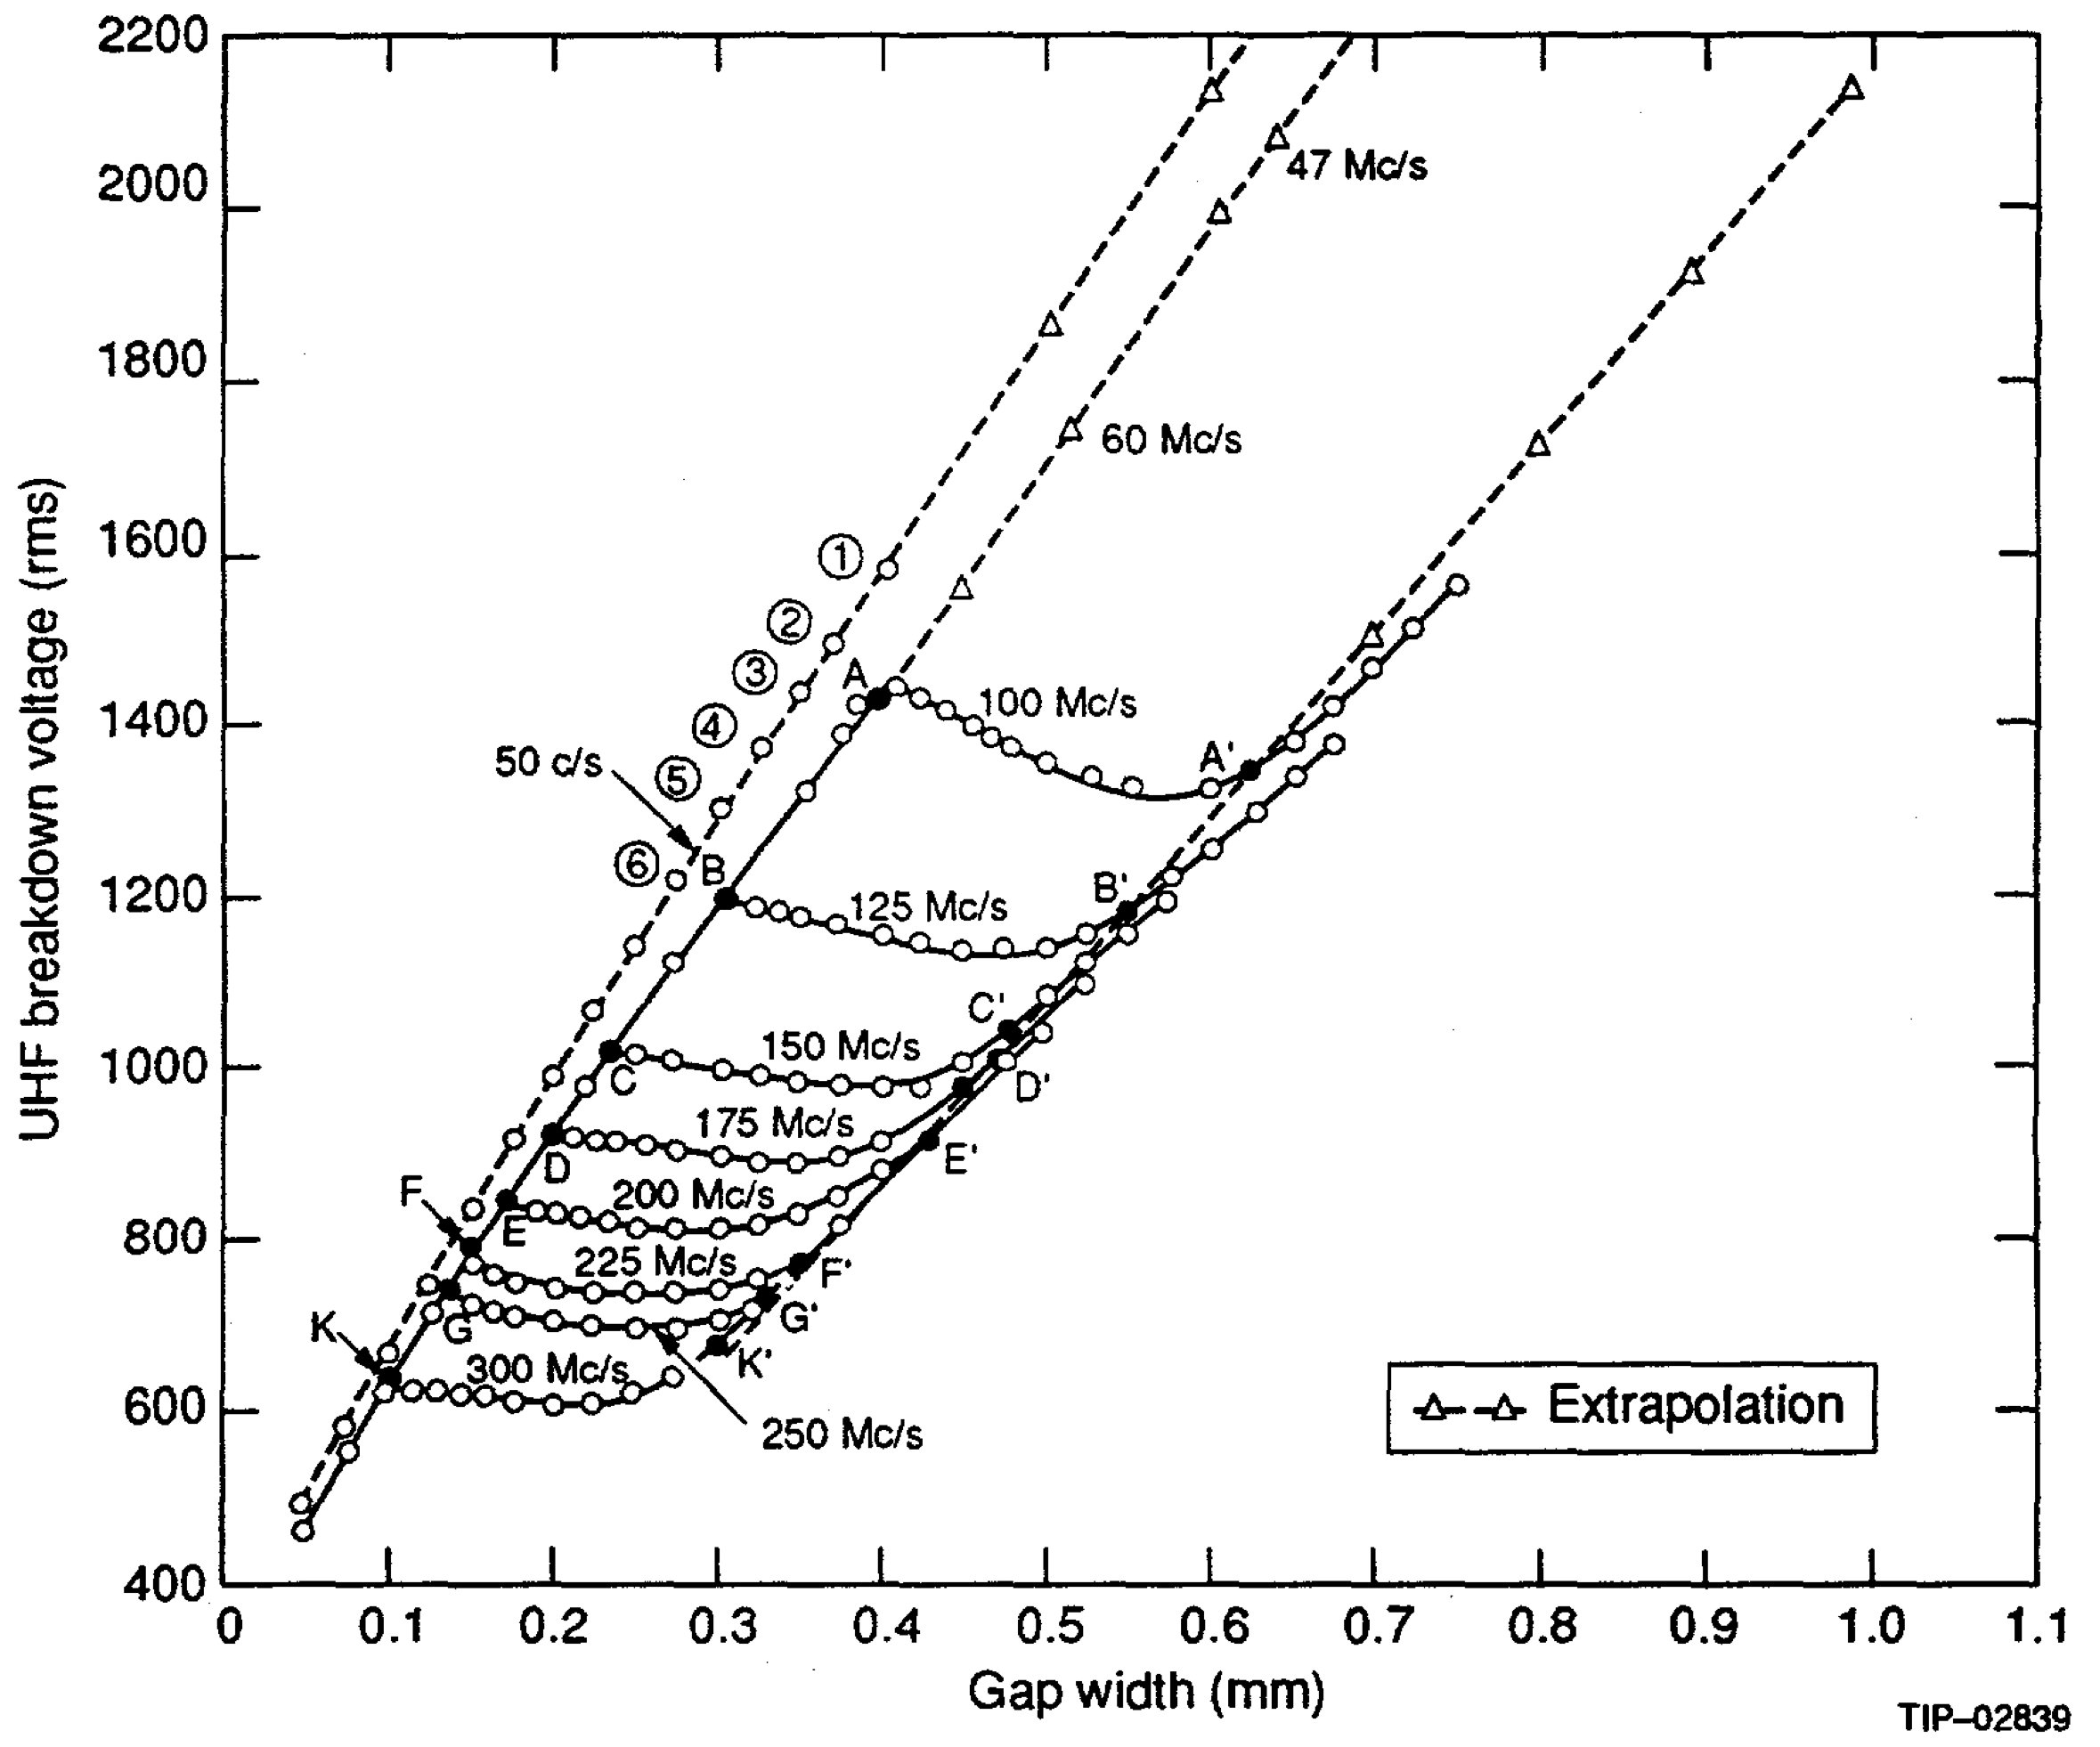
\includegraphics[width=\linewidth]{background/figures/ac_breakdown.png}
	\caption{Paschen curve for AC discharge across various frequencies \cite{Pim1949}.}
	\label{fig:ac_breakdown}
\end{figure} 


\section{Electron Beam Guns}

\subsection{DC-based Devices}

As seen in the previous section, a parallel plate configuration is one possible geometry to produce a electrons via a DC discharge. Another commonly used alternative is the hollow cathode geometry. Hollow cathodes are typically cylindrical in nature, where the anode remains the same but the cathode has been replaced with cup-like shape that is hollow in the centre (hence the name). Nonetheless, other designs are possible with examples of square hollow cathode developed by Fukuda et al \cite{Fukuda1998} and also tapered cathode shapes by Ohtsu et al \cite{Ohtsu2013}. In truth, the exact hollow cathode geometry to be used highly depends on the intended use case as each design has its pros and cons.

\begin{figure}[h!]
	\centering
	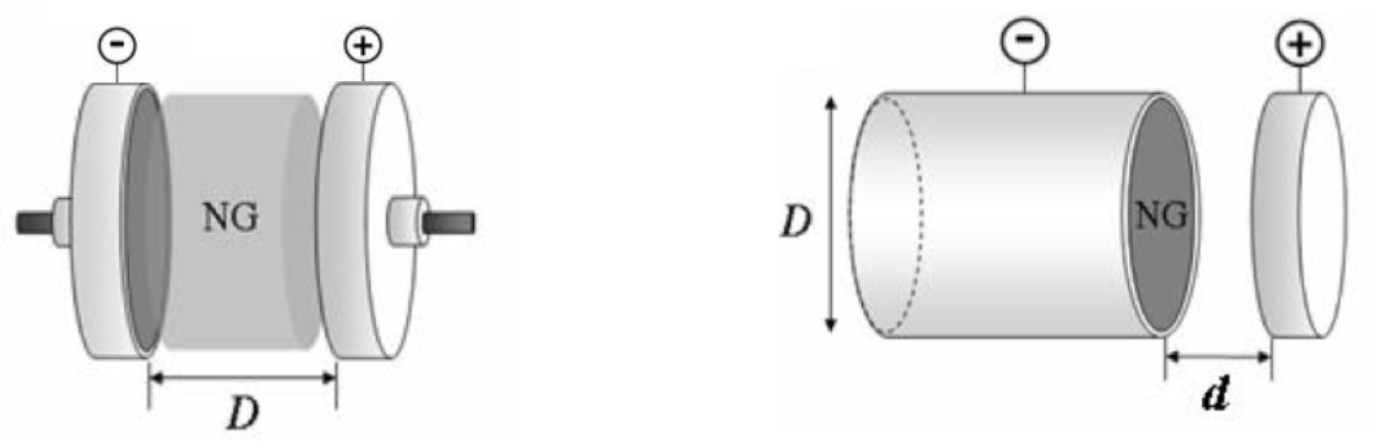
\includegraphics[width=0.8\linewidth]{background/figures/hollow_cathode.png}
	\caption{Comparison between a parallel plate (left) and a hollow cathode (right) \cite{Pessoa2007}.}
	\label{fig:hollow_cathode}
\end{figure} 

Despite the designs used, all hollow cathodes take advantage of a phenomenon known as the \textit{hollow cathode effect}. There are multiple factors that contribute to the hollow cathode effect. However, it is generally agreed upon that the primary mechanism is caused by the pendulum effect of electrons. Electrons, generated via secondary-emissions from the cathode, tend to oscillate back and forth between the cathode walls. This motions of electrons increases the likelihood that any given one will undergo an ionising collision with a neutral gas atom \cite{Arslanbekov1998}. This is quite similar to the behaviour of of AC discharge mentioned in section 2.1.3, however the difference being it only oscillates between the single electrode. The downside of this behaviour is that there tends to be excess heating of the cathode and increased potential of sputtering from ion bombardments on the cathode. However, these drawbacks can be minimised by carefully selecting design and operating conditions of the device. The benefits over a parallel plate geometry are that hollow cathodes tend to have a lower breakdown voltage (particularly at low gas pressures) \cite{Kolobov2015, Eichhorn1993} compared to their parallel plate counterparts. Additionally, they generally produce a higher current density for a given operating voltage \cite{Kolobov2015, Pillow1981}. As such, it is the hollow cathode design that is the preferred geometry for a plasma-cathode electron gun.

An example of a hollow cathode based electron gun can be in figure \ref{fig:kornilov_device}. This device was developed by Kornilov et al \cite{Kornilov2009}, and can be divided into two separate sections: the discharge region and acceleration region. 

\begin{figure}[h!]
	\centering
	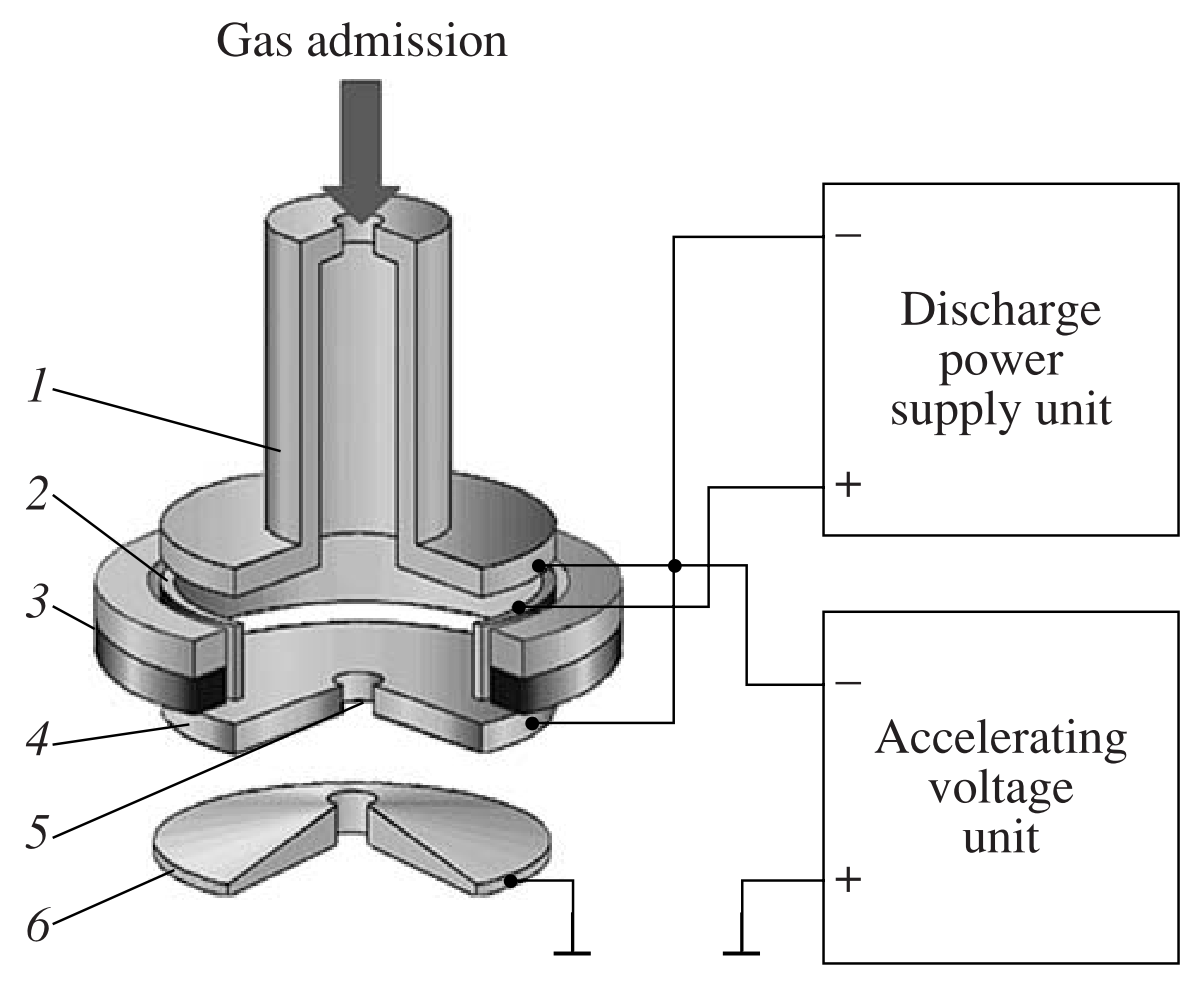
\includegraphics[width=0.6\linewidth]{background/figures/kornilov_device.png}
	\caption{Electron Gun Design by Kornilov et al \cite{Kornilov2009}: (1) hollow cathode, (2) anode, (3) permanent magnet, (4) auxiliary electrode (emidng cathode), (5) emission channel, and (6) accelera8ng electrode.}
	\label{fig:kornilov_device}
\end{figure}

The electrodes (1 and 2) used in the discharge region. There are two key differences seen here compared to the hollow cathode shown previously. First and foremost is that the anode takes the shape of a ring rather than a plate, which is to simply to allow the electrons generated to exit the discharge region. The other difference is the presence of an inlet at the top of the cathode. This allows a constant stream of gas feed to replenish the gas that has been ionised. This gas feed also ensures that pressure within the discharge region remains roughly constant, at about 1-10 Pa. There is also a permanent magnet (3) used to focus the beam into the emission channels (5). As for the accelerating region, there are two addition electrodes (4 and 6) with a high voltage applied to accelerate beam out of the gun. The pressure in the acceleration is kept quite low, at around 0.01 Pa. This mitigates electric charges within the gun and also prevents the focused beam from diverging. 

The device by Kornilov et al produced an electron beam with a diameter roughly 260um. This was achieved with a power of 3kW to the overall gun. The potential difference for the discharge electrodes were approximately 350-450 V, whilst the voltage at the accelerating electrodes were on the order of 30 kV. 

Some other approaches for designing an electron gun exists, such as the one developed by Bakeev et al \cite{YuBakeev2018} seen in figure \ref{fig:bakeev_device}. This design forgoes the accelerating region, instead relying on much higher voltages for the discharge electrodes. This was between 20-30 kV. The pressure of the discharge region was also higher, at around 10-30 Pa.

\begin{figure}[h!]
	\centering
	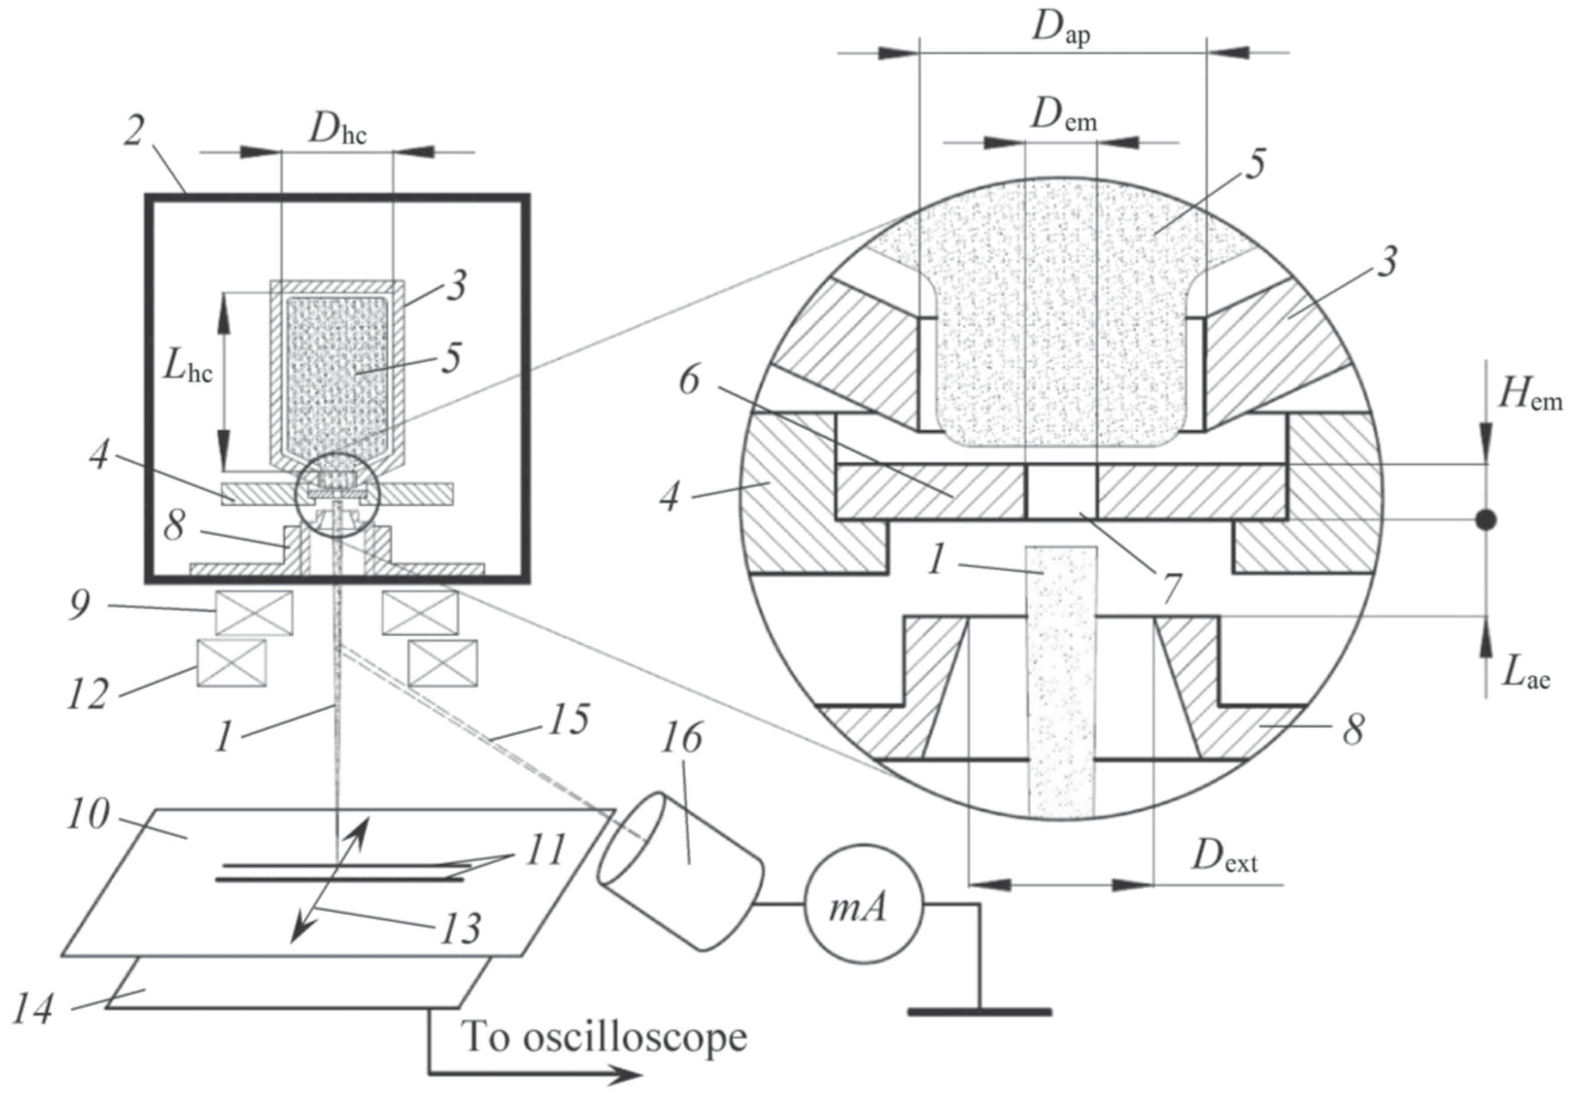
\includegraphics[width=0.6\linewidth]{background/figures/bakeev_device.png}
	\caption{Electron Gun Design by Bakeev et al \cite{YuBakeev2018}: (1) electron beam, (2) enclosure to maintain forevacuum-pressure, (3) hollow cathode, (4) anode, (5) emission plasma, (6) metal disk, (7) emission channel, (8) extractor, and (9) focusing magnetic system. (Note: the un-labelled components were for testing the beam.)}
	\label{fig:bakeev_device}
\end{figure}

One of the biggest differences in this design was that the hollow cathode was that the aperture of the hollow cathode was reduce to a gap of 8 cm. This was done to improve the electron extraction efficiency, and as a result the hollow cathode was less cup-shaped and more akin to a water bottle. Another difference is that magnets used for focussing the electron beam were located outside the gun itself. This could possibly because the hollow cathode design used already focused the electron beam out of the gun, hence the magnets are only necessary to obtain a smaller beam diameter. The final diameter of the electron beam was 200 um.  


\subsection{AC-based Devices}

Because an AC-based plasma does not rely on the secondary emissions from the cathode, the utilisation of a hollow cathode design is not strictly necessary. Despite that, the general structure of the AC electron guns do share a number of similarity to their DC-based counterparts.

An example of a radio frequency (RF) plasma cathode electron gun can be seen in figure \ref{fig:del_pozo_device}, developed by Del Pozo et al \cite{Pozo2014}. In the figure \ref{fig:del_pozo_device}, there are a number of parts that pertain to the RF circuit, however the components within the plasma device (seen in the dashed outline 12) are quite familiar. 

\begin{figure}[h!]
	\centering
	\begin{subfigure}[b]{0.7\linewidth}
         \centering
         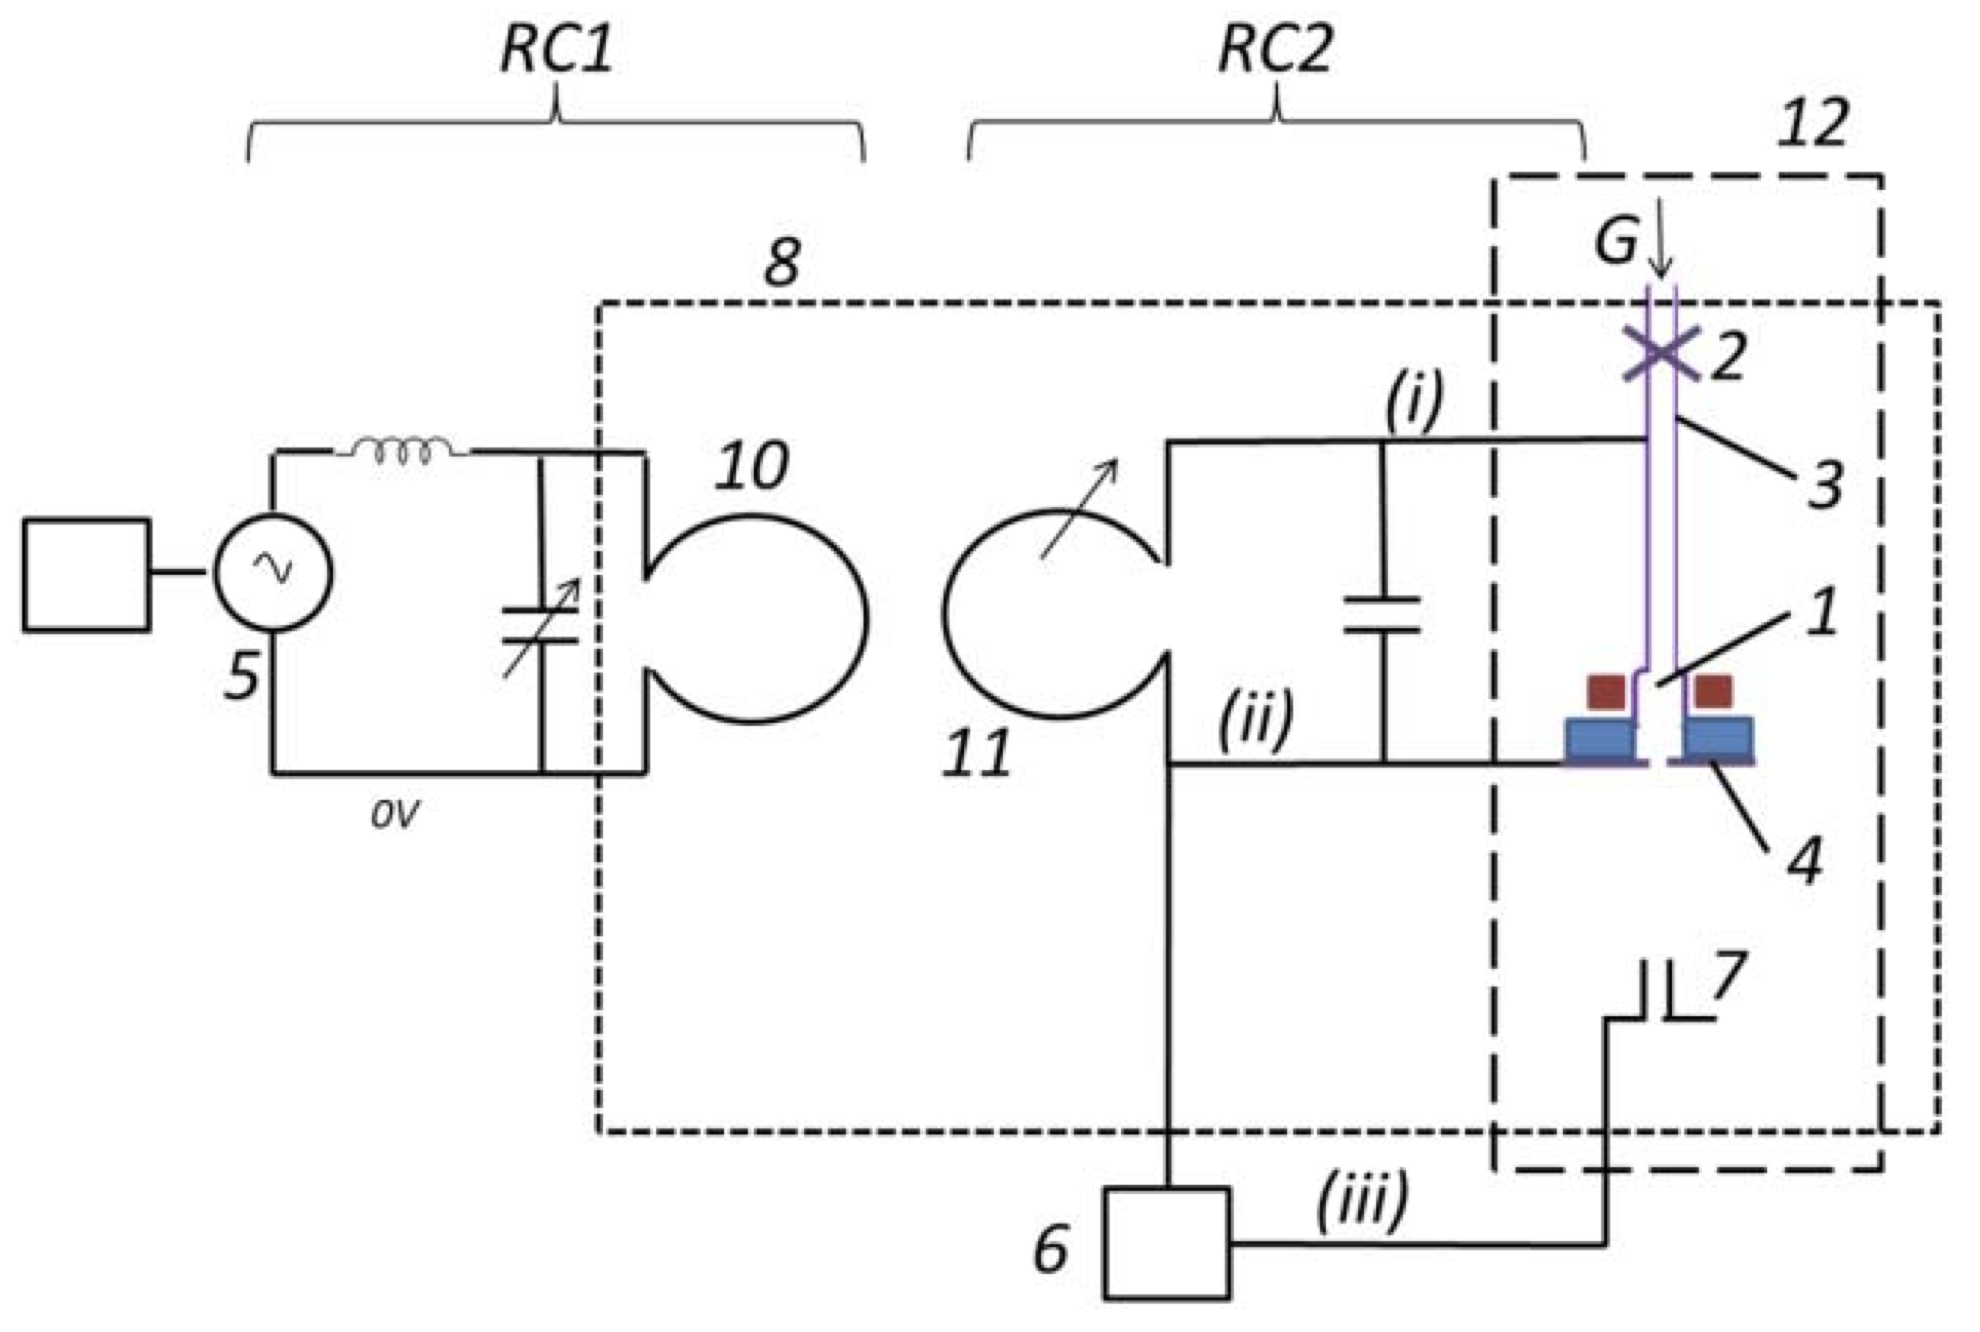
\includegraphics[width=\linewidth]{background/figures/del_pozo_device.png}
         \caption{Circuit schematic.}
     \end{subfigure}
     \begin{subfigure}[b]{0.7\linewidth}
         \centering
         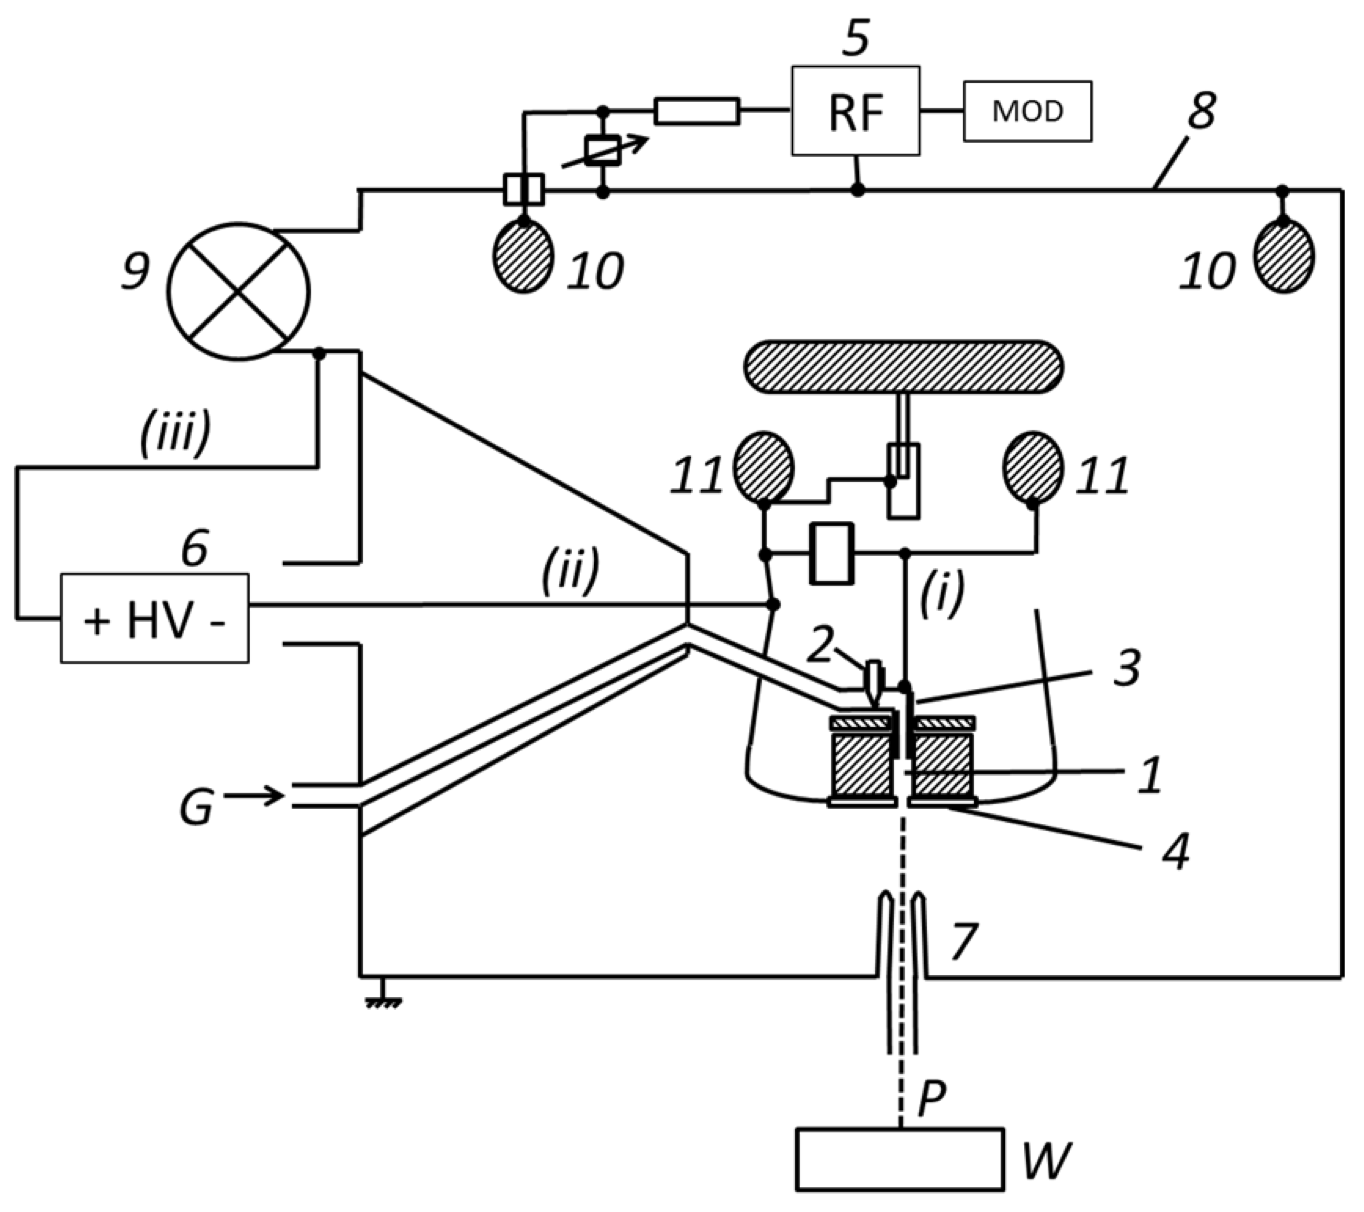
\includegraphics[width=\linewidth]{background/figures/del_pozo_device_2.png}
         \caption{Cross section of device.}
     \end{subfigure}
	\caption{Electron Gun Design by Del Pozo et al \cite{Pozo2014}: 
	a plasma chamber (1) gas feed inlet, (2) gas valve, (3 and 4) discharge electrodes, and (7) accelerating electrodes.}
	\label{fig:del_pozo_device}
\end{figure}

For the RF plasma device, there was a gas feed inlet (2) that maintains a relatively high pressure within the plasma chamber (1), between 10-100 Pa. There were also two sets of electrodes. The first set are the discharge electrodes (3 and 4) designed for frequency of 84 MHz. The generated electrons then exit the plasma chamber into the accelerating electrodes. These electrodes had a very large voltage of -60 kV, and t ow pressure of 0.01 Pa in order to ensure the electrodes were electrically isolated.

